\section{Automatisierte Tests}
Während der Entwicklung wurden diverse automatisierte Tools verwendet, welche direkt mit der Versionskontrollsoftware
verbunden waren. Dadurch wurde jeder Commit mit den beschriebenen Tools (siehe Tabelle \ref{qs_tools}) überprüft.
\begin{table}[H]
	\centering
	\begin{tabular}{|l|p{18em}|l|}
		\hline
		\textbf{Tool} & \textbf{Beschreibung} & \textbf{Notwendig für...} \\\hline
		AppVeyor & Ausführung von Unittests unter verschiedenen Windowsversionen & Portabilität, Korrektheit \\\hline
		Codacy & Überprüfung der Codequalität basierend auf Styleguides der verschiedenen Sprachen& keine \\\hline
		Travis CI & Ausführung von Unittests unter verschiedenen Linux- und Pythonversionen & Portabilität, Korrektheit \\\hline
		coveralls & Überprüfung der Testabdeckung & Korrektheit \\\hline
		pyup.io & Überprüfung der verwendeten Bibliotheksversionen auf Updates & keine \\\hline
	\end{tabular}
	\caption{Automatisierte Tools für die Qualitätssicherung}
	\label{qs_tools}
\end{table}

Durch die Integration in die Github-Infrastruktur wurde für jeden Pull-Request (in unserem Modell entsprach ein Pull-Request einer Userstory)
ein entsprechender Report generiert (Beispiel in Abbildung \ref{github_checks}).

\begin{figure}[h]
	\centering
	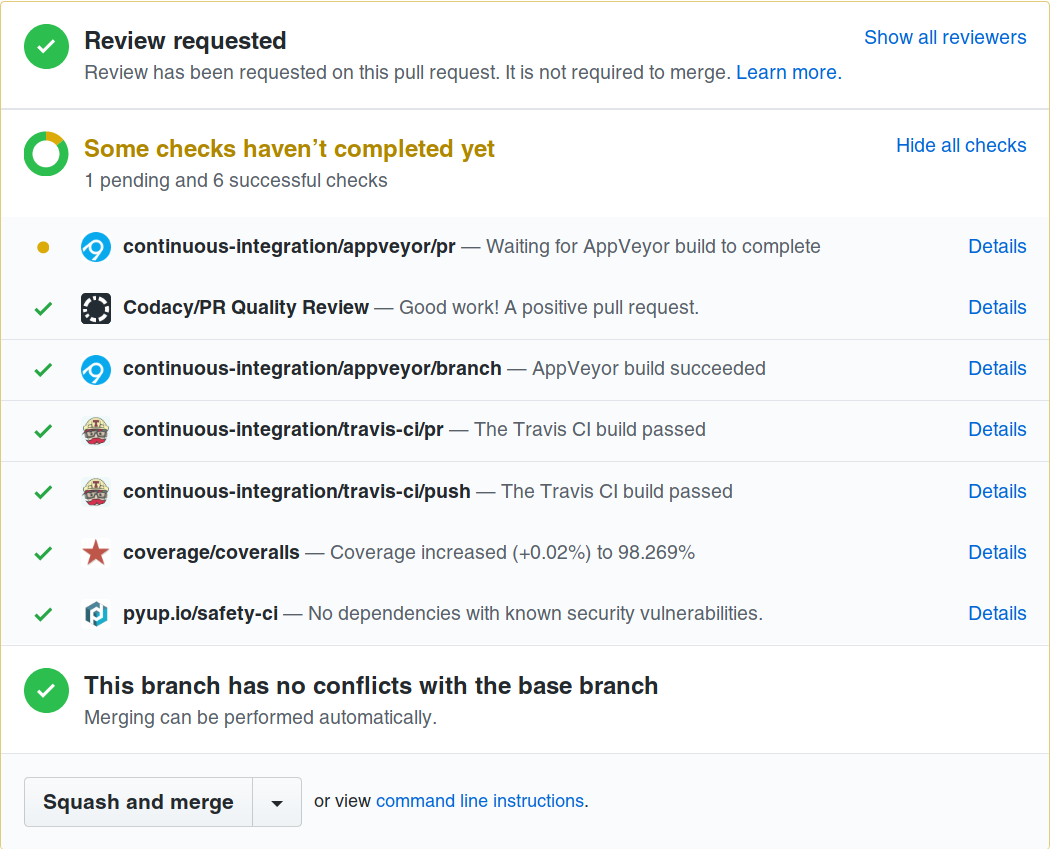
\includegraphics[width=.7\textwidth]{github_checks}
	\caption{Übersicht der durchlaufenden Checks}
	\label{github_checks}
\end{figure}

Die Unittests, welche von AppVeyor und Travis CI ausgeführt wurden, deckten große Teile des Python Codes ab. Sie sind im Github Repo
zu finden\footnote{\url{https://github.com/bp-flugsimulator/server/tree/master/frontend/tests}} und aufgrund ihrer Anzahl (~200) nicht
Teil des Anhangs.
Die Abdeckung lag immer bei über 90\% und war ein Kriterium für die Abnahme einer Userstory. Eine Übersicht der Abdeckung
findet sich in Abbildung \ref{coverage_pdf}.
Die Tests fanden unter folgenden Umgebungen statt:
\begin{itemize}
	\item Windows (Windows Server 2016, jeder Test mit 32 und 64 Bit Versionen)
		\begin{itemize}
			\item Python 3.4
			\item Python 3.5
			\item Python 3.6
		\end{itemize}
	\item Linux (Ubuntu, 64 Bit)
		\begin{itemize}
			\item Python 3.4
			\item Python 3.5
			\item Python 3.6
		\end{itemize}
\end{itemize}
\begin{figure}[t]
	\centering
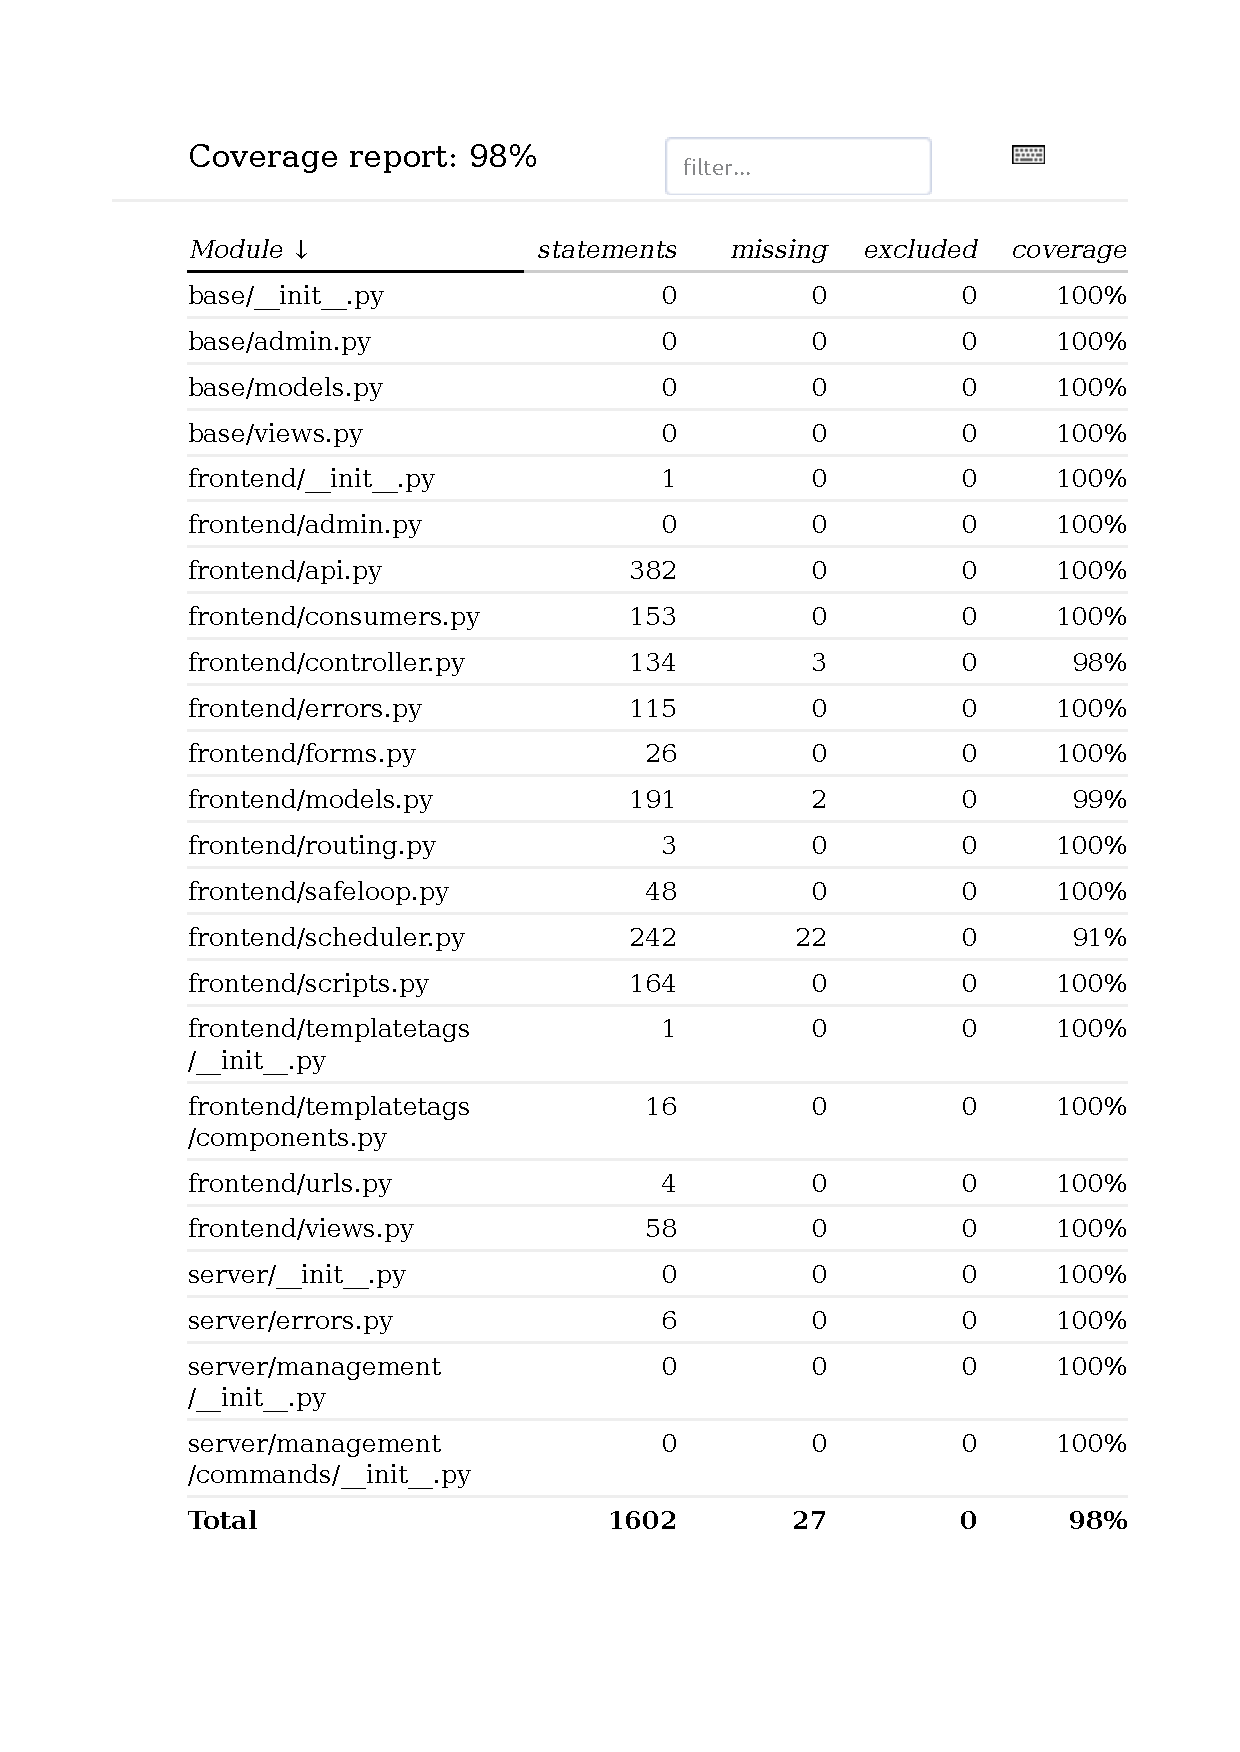
\includegraphics[width=.8\textwidth]{img/coverage.pdf}
	\caption{Abdeckungsübersicht am Ende des Projekts}
	\label{coverage_pdf}
\end{figure}
Der Stand von Codacy zum Ende des Projekts findet sich in Abbildung \ref{codacy_png}. Während
es keine stilistischen Fehler gibt ('Issues 0\%'), gibt es sehr viel doppelten Code, da viele Methoden
in der API einen ähnlichen bis gleichen Anfang haben.

Ein erfolgreicher Testrun von Travis\footnote{\url{https://travis-ci.org/bp-flugsimulator}} ist in Abbildung \ref{travis_png} zu sehen, von AppVeyor\footnote{\url{https://ci.appveyor.com/project/GreenM0nst3r/server/history}} in Abbildung \ref{appveyor_png}.
Die Ergebnisse finden sich unter 


\begin{figure}[t]
	\centering
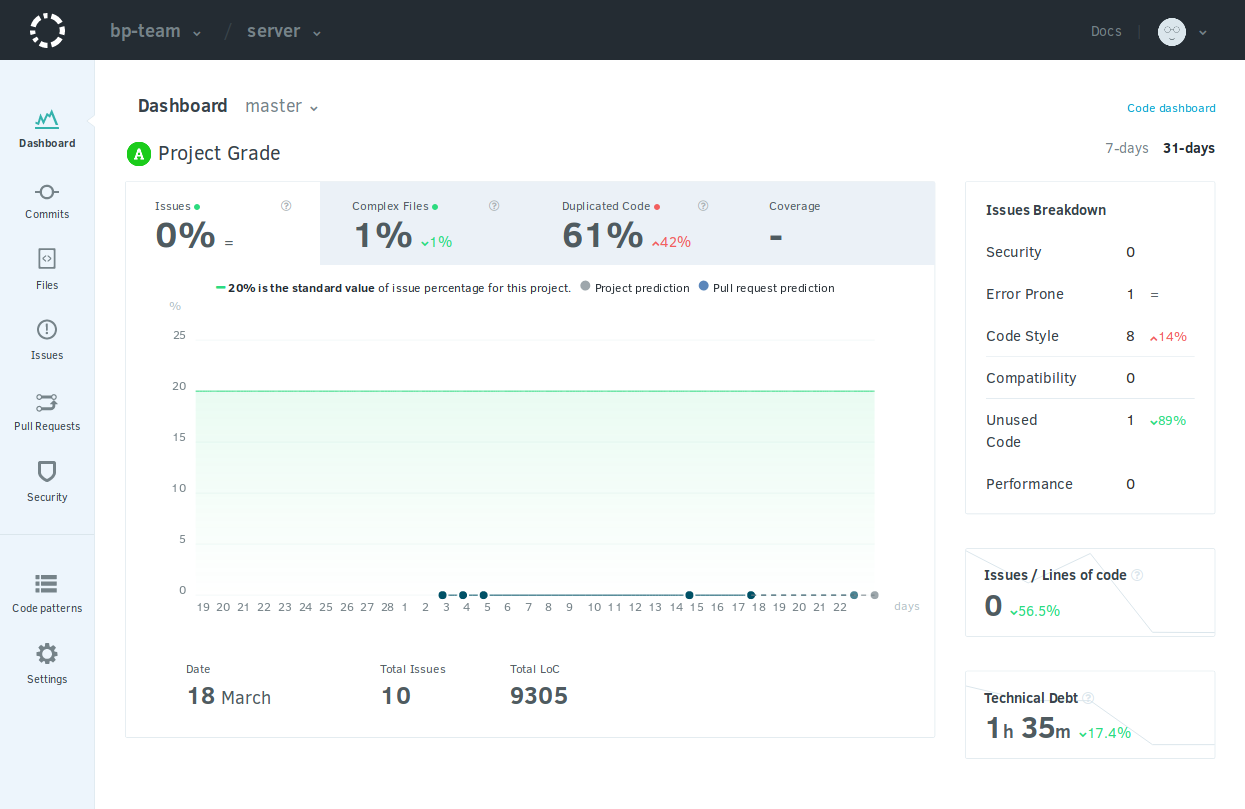
\includegraphics[width=.9\textwidth]{codacy}
	\caption{Stilüberprüfung am Ende des Projekts}
	\label{codacy_png}
\end{figure}

\begin{figure}[h]
	\centering
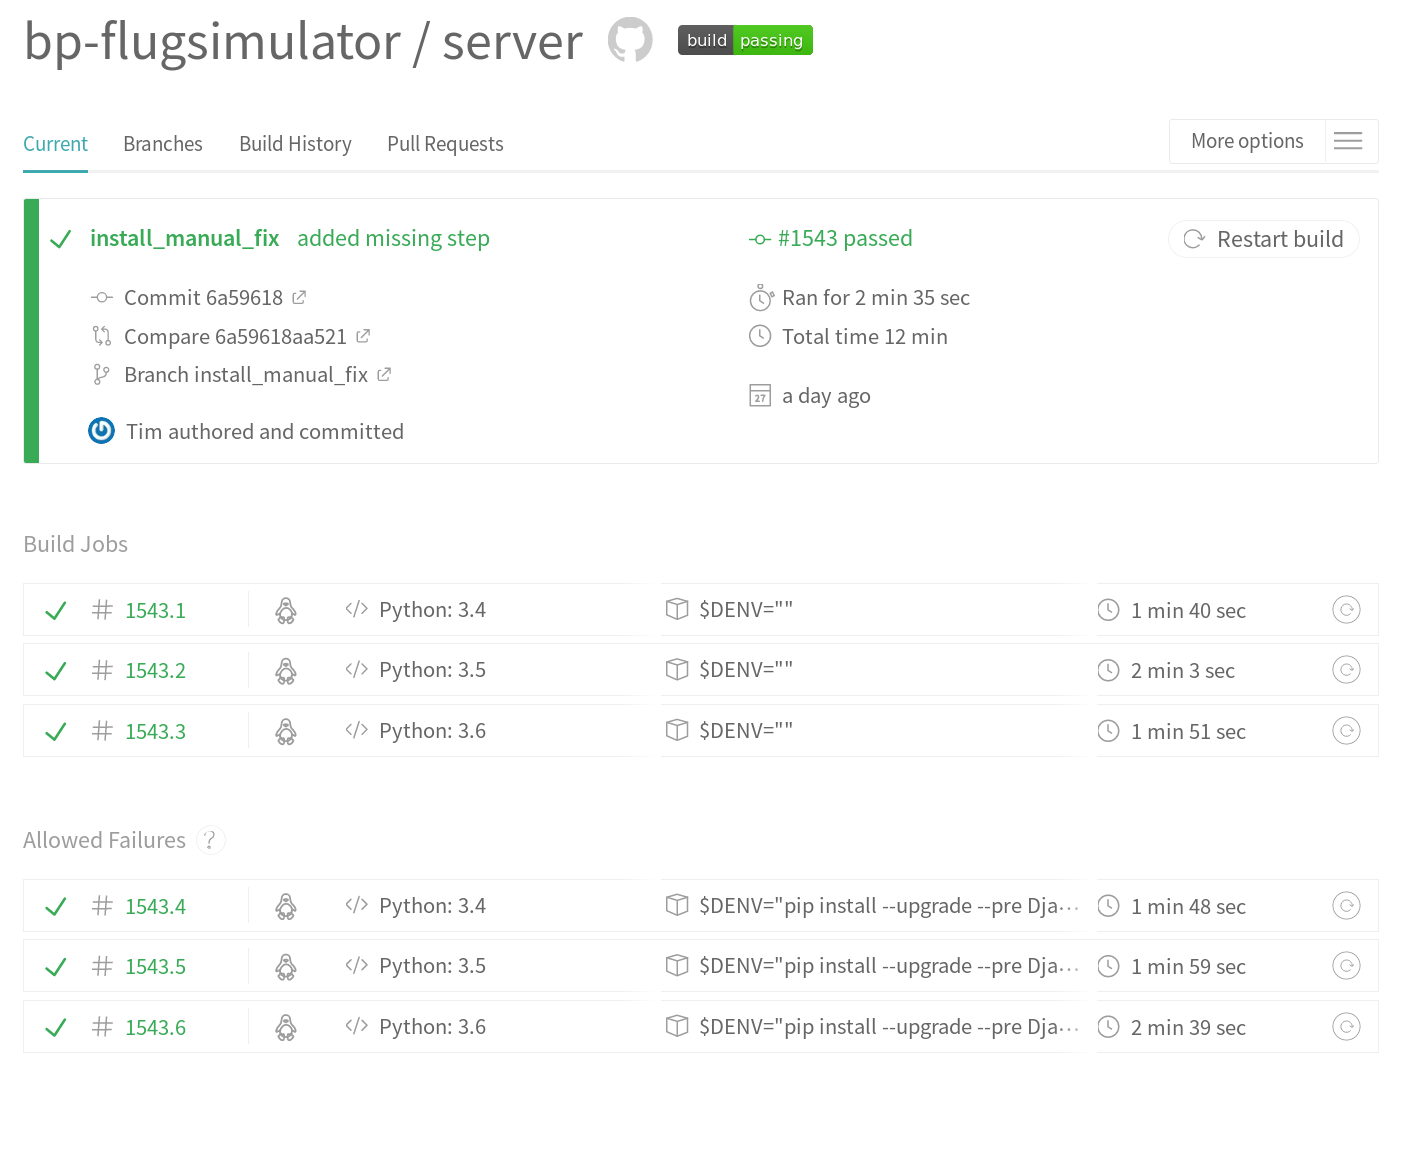
\includegraphics[width=.9\textwidth]{travis}
	\caption{Erfolgreicher Testdurchlauf von Travis}
	\label{travis_png}
\end{figure}

\begin{figure}[h]
	\centering
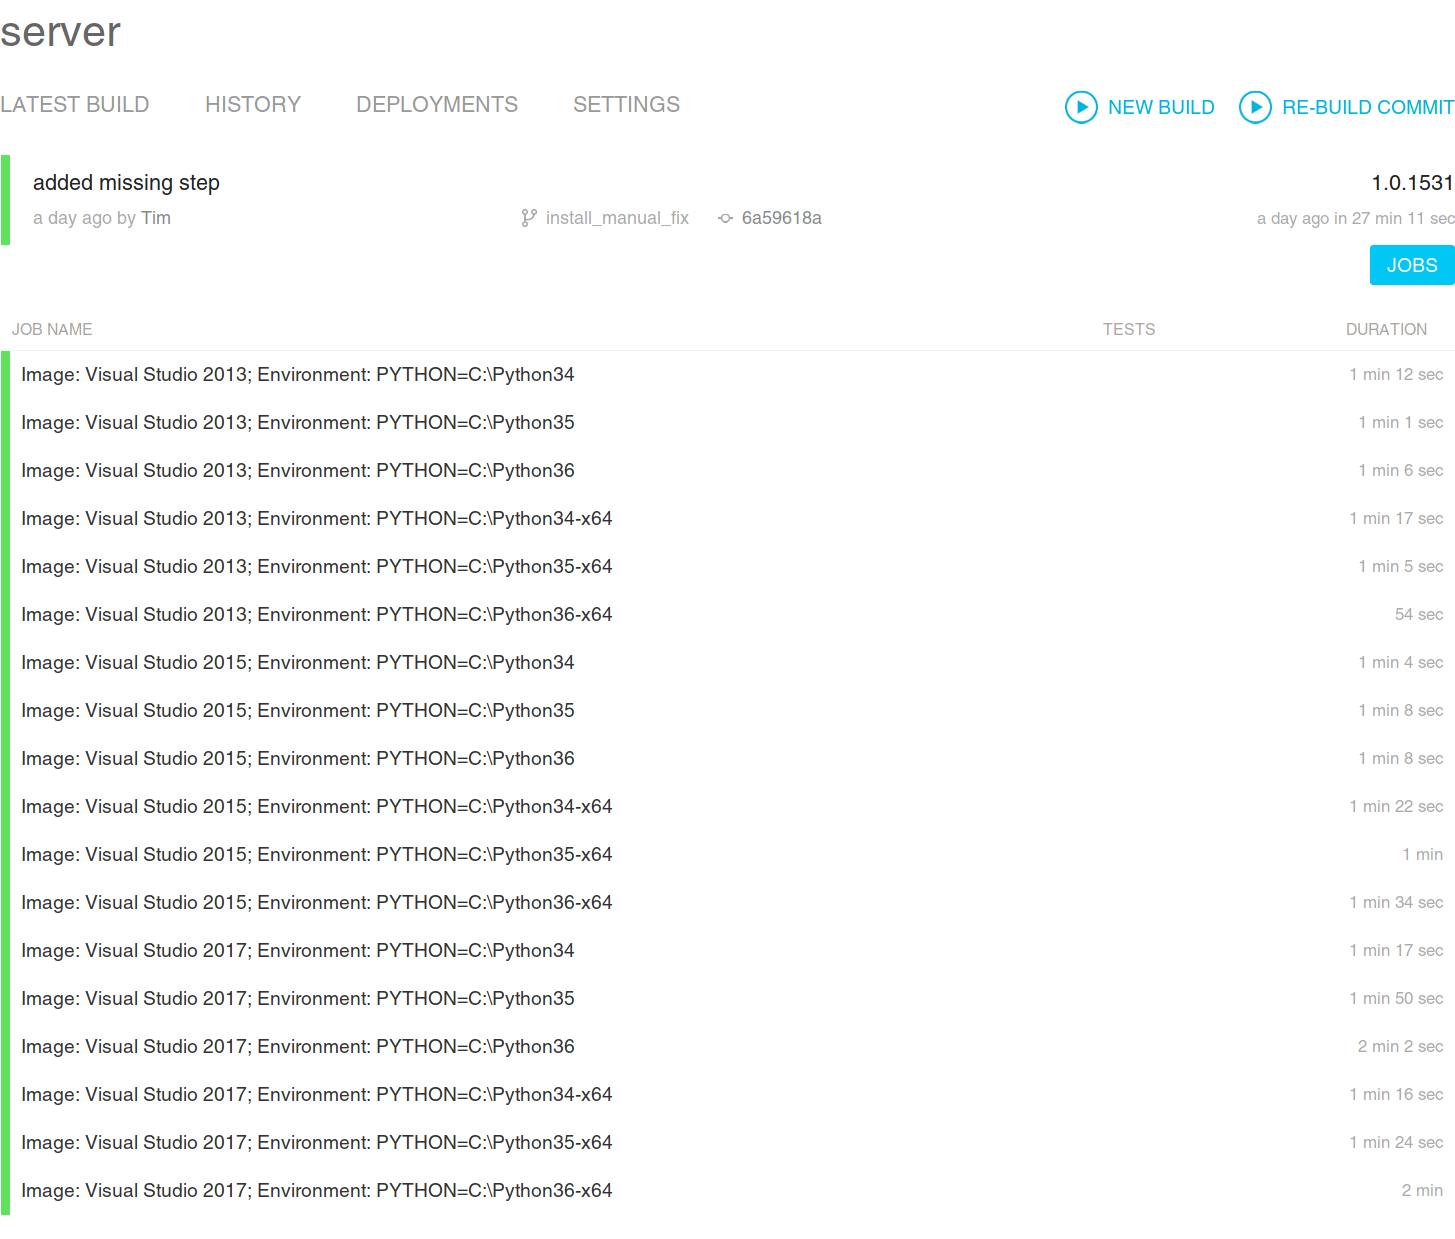
\includegraphics[width=.9\textwidth]{appveyor}
	\caption{Erfolgreicher Testdurchlauf von AppVeyor}
	\label{appveyor_png}
\end{figure}
